The fi rst domain we consider is modeling and simulation.

Dave Moursund [6] suggests “the underlying idea in computational think- ing is developing models and simulations of problems that one is trying to study and solve.

”In Project GUTS (Growing up Think- ing Scientifi cally) middle school students actively engage in computational thinking as they design and implement models of local relevance and then use the models to run simulations.

Students used the process of abstraction to narrow the problem down to something that could be implemented on the computer using StarLogo TNG, an agent based modeling tool.

Restrictions imposed by the model- ing environment include an upper bound on the number of agents (4076) and a limit on the size of the environment (101 by 101 cells).

Within these parameters students designed and created models as testbeds to answer questions about real-world concerns.

For example, as part of the Project GUTS unit on Epidemiology, a group of students wanted to know if a disease would spread throughout their school population given the layout of the school, the number of students, the movement of the students, the virulence of the disease, and the number of students initially infected.


A atividade em questão foi reportada por \citeonline{Lee2011}, na qual um grupo de estudantes elaboram um modelo epidemiológico com o propósito de investigar se uma doença poderia se espalhar entre a população escolar em função do layout da construção, do número e movimento dos estudantes, da virulência da doença e do número de pessoas inicialmente infectados.
 
Para o mapeamento desses fatores no modelo foi utilizado um software de modelagem baseado em agentes (entidades ou atores com liberdade de movimento espacial, geralmente bidimensional, definida por regras previamente estabelecidas) chamado \textit{StarLogo TNG}\footnote{Disponível em \href{http://web.mit.edu/mitstep/starlogo-tng/download/index.html}{http://web.mit.edu/mitstep/starlogo-tng/download/index.html}} (fig. \ref{fig:starlogo}).

\begin{figure}[!htb]
  \caption{Imagem do software de modelagem Starlogo, desenvolvido pelo \text{MIT Media Lab}}
  \begin{center}
    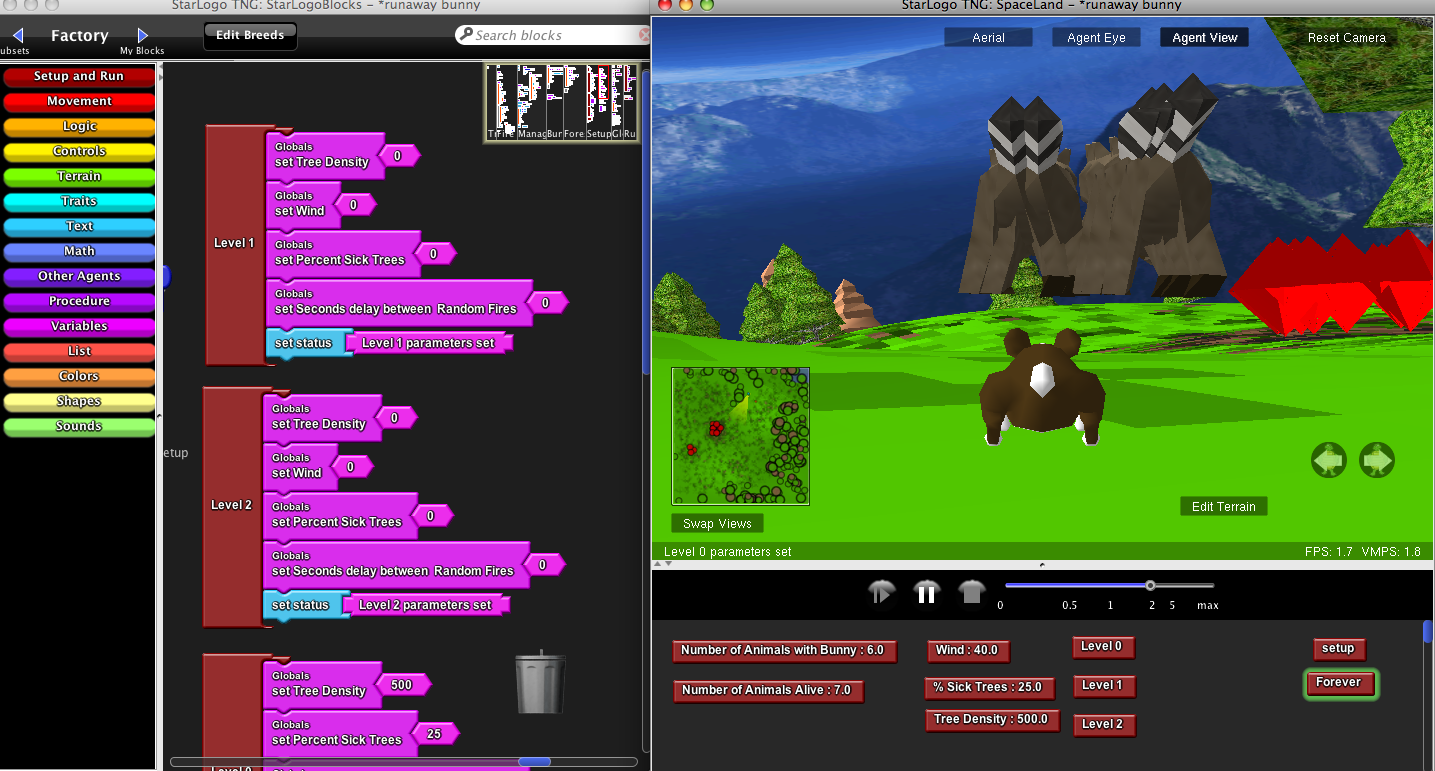
\includegraphics[width=0.8\textwidth]{imagens/starlogo}
  \end{center}
  \label{fig:starlogo}
\end{figure}

Durante execução desta atividade tais agentes foram tomados como uma abstração dos estudantes, e a quantidade inserida no modelo correspondeu à exatamente ao de matriculados na escola. O movimento atribuídos às entidades teve por finalidade a criação de uma representação simplificada do movimento dos alunos de uma sala a outra. Já a delimitação espacial do ambiente buscou a reprodução do espaço físico da instituição. A elaboração deste modelo está ilustrado na imagem

\begin{figure}[!htb]
  \caption{}
  \begin{center}
    \includegraphics[width=0.8\textwidth]{imagens/layout-startlogo}
  \end{center}
  \label{fig:starlogo}
\end{figure}


See Figure 1.

Mapping this question and scenario onto an agent based model, agents were used as abstractions or simplified representations of stu- dents and the number of agents matched the number of students in their school.

Agents were given movement behaviors that were abstractions of moving from classroom to classroom, and decisions were made about which features of the school were important to take into consideration before a 3-D virtual model of the school building was created.

For instance, students decided that recreating the num- ber and location of passages and doors at the school was important.

Additionally students modeled the characteristics of the contagion being spread: how often contact between students spread the disease from one to the other and how many students were initially infected.

To make the model a testbed capable of running experiments, it was equipped with interface sliders to control individual variables.

One slider controlled the number of initially infected agents and another controlled the virulence of the contagious element.

See Figure 2.
 

Automation was used in a number of ways.

The “program” itself automated “stepping through” or advancing the simulation through the use of a run loop that updated each agent’s state, location, and color (representing sick or healthy) at each time step.

Because agent-based models involve randomness, for example, the initial location of infected individuals is chosen randomly, they tell us the probabilities of certain outcomes rather than predictions.

Automa- tion was used to execute multiple “runs” of the experiment with the same parameter settings in order to attain the probabilities of certain outcomes.

Once the simulations were run and data on the number of infected individuals after a fi xed number of time steps were collected, students refl ected on the outcomes.

In some cases, the students were able to analyze their models, the assumptions and abstractions made, by comparing the model generated data with data collected within their schools.

For instance, one group compared the data generated using their model that simulated the spread of swine flu with attendance/absenteeism records collected during a period of time when swine fl u was known to be circulating within their school.

Analysis of this sort may lead to reconsideration of what factors to include in a model and cycle back to the beginning of the process described above.

